% !Mode:: "TeX:UTF-8"
\chapter{H.265 帧内无损编码 FPGA 原型验证平台}
\label{cha:c5}
当电路系统复杂度高于一定程度时,传统的行为级仿真已经难以满足设计的验证需求,使用 FPGA 进行原型验证灵活度高,验证结果可靠,且有利于软硬件协同设计、加快项目开发进度。因此 FPGA 原型验证成为了复杂系统 ASIC 化之前不可或缺的一个步骤。本课题亦完成了一 FPGA 原型验证平台,对硬件编码系统进行验证。

\section{FPGA 原型验证方案}
为了对设计的硬件编码器进行验证,本课题设计、搭建了一个完整的 FPGA 原型验证平台。该验证平台由视频源、预处理模块、通信模块、硬件编码器和上位机解码模块组成。利用该平台可实时编码由视频源提供的图像信息,经映射入 FPGA 的硬件编码器编码后将码流传回上位机,在上位机对码流进行网络适配层码流的拼接后,由上位机软解码,实时查看软解码结果正确与否即可对硬件编码器进行验证。完整的验证平台如图 \ref{fig:FPGADemoBlock} 所示。
\begin{figure}[hbt]
    \centering
    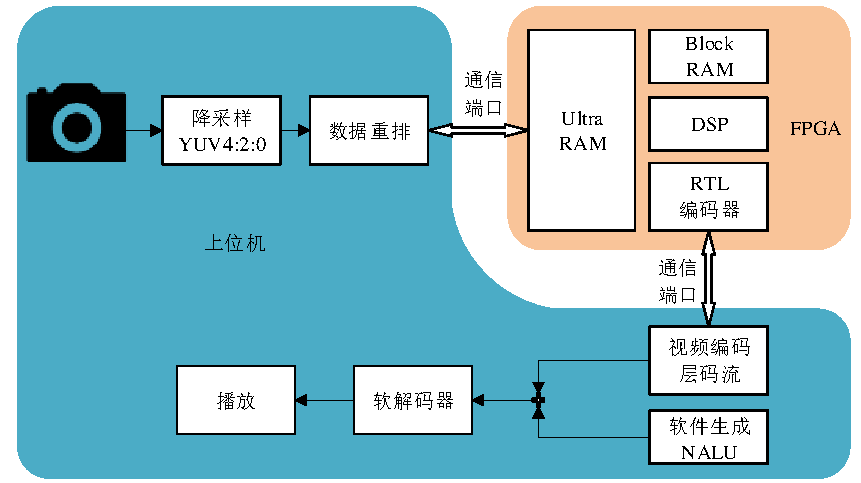
\includegraphics{FPGADemoBlock.pdf}
    \caption{FPGA 原型验证平台}
    \label{fig:FPGADemoBlock}
\end{figure}

\section{FPGA 验证平台关键模块}
验证平台由上位机与 FPGA 共同组成,上位机进行视频源的获取与预处理,同时负责对 FPGA 输出的码流进行加工、软解码,最终实时播放;FPGA 负责映射硬件编码器,其中使用大量的专用存储器资源实现数据缓存和交换,以保证留出足够的查找表实现编码逻辑的映射。通信端口由上位机和 FPGA 共同处理,根据通信速率的需求可选择串口、以太网口甚至 PCI-E 接口进行通信。
\subsection{FPGA 器件}
FPGA 原型验证平台所使用的器件是基于 XILINX Zynq UltraScale+ MPSoCs 开发平台的开发板 AXU15EG。主芯片为 XCZU15EG-2FFVB1156I,外挂 2GB DDR4。底板扩展了外围接口,本课题所设计的部分包括 USB3.0 接口、千兆以太网接口、UART 接口、FMC 接口、RS485 接口以及 MIPI 接口。所用器件的完整结构如图 \ref{fig:FPGAIntroduce} 所示。
\begin{figure}[hbt]
    \centering
    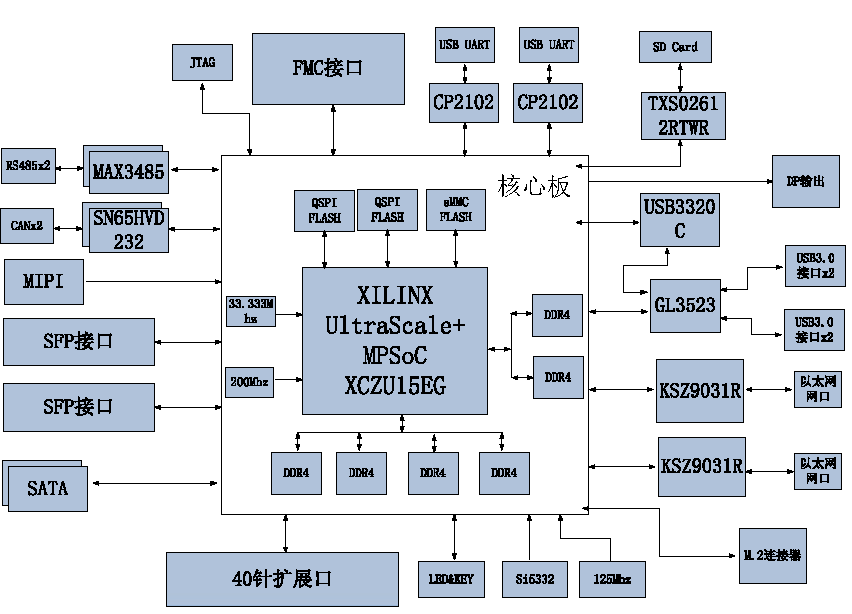
\includegraphics{FPGAIntroduce.pdf}
    \caption{FPGA 器件完整结构}
    \label{fig:FPGAIntroduce}
\end{figure}

\subsection{视频源及预处理}
原型验证平台的待编码视频源可有多种形式,灵活适用于不同场景。
\begin{enumerate}
    \item 视频文件

          使用上位机中存储的视频文件作为视频源。其方便提供、数据内容固定的特性使该方式多用于严谨的编码器性能统计、分析。另外,由于不存在与其余硬件的交互,可将开发过程中的不确定性控制在最小,因此也多用于 FPGA 的仿真验证阶段。

    \item HDMI 输入

          使用显卡或工业相机的 HDMI 输出流作为视频源。FPGA 可与 FMC 视频扩展子板组合使用,直接将 HDMI 差分信号转换为 RGB 信号。但由于 HDMI 信号几乎无法在上位机进行预处理,需要在硬件部分进行降采样、重排序等操作,对前期平台搭建十分不利,无法定位问题出现的模块。因此该方案一般用于验证平台成熟后的扩展。

    \item USB 相机输入

          使用 USB 相机的输出流作为视频源。USB 相机可通过直接连接在上位机的形式提供视频源,并且直接在上位机进行各类预处理,以保证 FPGA 器件上的工作只有编码和通信,最大程度上地减少了硬件验证地不确定性。此外,由于视频源率先存储在上位机,故可将待编码帧暂存,待收到 FPGA 器件地输出码流后进行软解码并与视频源做对比,统计出 PSNR 等各类信息。综上所述,FPGA 验证平台选用 USB 相机作为输入。
\end{enumerate}

预处理是上位机需要进行的操作之一。预处理包括色彩格式转换、降采样和数据重排。
\begin{enumerate}
    \item 色彩格式转换

          大部分视频输出设备的输出色彩格式是 RGB,因为 RGB 通道格式最适合各类显示器显示。但在视频编解码领域,最常使用的是 YUV 色彩通道,即亮度-色差通道。因为 YUV 格式天然地将人眼不同敏感程度的色彩分量区分了出来,因此可在编码过程中人为的将色差通道进行高失真高编码效率的处理而不产生明显的视觉损失。色彩格式转换在 FPGA 平台上实现需要消耗大量的中间缓存存储器,为了给复杂的 H.265 编码器留出资源,将色彩格式转换转移到上位机中进行。

    \item 降采样

          通常来说,为了最大程度地提高编码效率,视频编码器直接处理的数据会经过降采样,即常见的 Y:U:V=4:2:0 格式,将色差通道的数据在水平和垂直方向上各降采样 1/2,经过降采样后待编码的数据量直接减少了 50\% 而不会产生明显的视觉损失。这一操作并不复杂,仅涉及到部分数据的舍弃,但与色彩格式转换类似需要消耗一定的存储器资源。且受到通信接口速率的限制,在 FPGA 平台上进行降采样直接影响了验证平台的吞吐率,因此将降采样转移到上位机中进行。

    \item 数据重排

          通常来说,测试视频序列与视频源输出存储的文件中,像素值的排列顺序属于平面模式,即在内存空间中按照 YYYYYYYY....UUUU..VVVV.. 的顺序,依次存放 3 个色彩空间的数据。然而在图像编解码中,由于其以编码块为基本单位的架构,编码器在处理数据时往往是按照块状空间进行的,且 YUV 3 个色彩空间的数据要求交替出现。因此硬件视频编码器中总是需要一块极大的存储器缓存视频源提供的数据。同样出于减轻 FPGA 不必要的资源消耗的目的,本原型验证平台将数据重排的任务交给上位机进行,数据通过通信端口进入 FPGA 后几乎只需要按照一般队列的模式顺序读取即可,极大地减小了 FPGA 资源消耗与 debug 难度。
\end{enumerate}

\subsection{与上位机通信接口}
% USB串口CP2102 以太网口 PCIE
通信接口是上位机与 FPGA 开发板通信的唯一渠道。根据使用场景的需求,可选择使用串口(USB2UART)或以太网口。
\begin{enumerate}
    \item 串口(USB2UART)

          UART 是极为经典的一种简单通信接口,以串行方式进行数据通信,以 1 周期的低电平表示数据开始发送。目前传统意义上的串口(RS232)因波特率过低,在学术界已很少使用,原型验证平台中 FPGA 的串口是通过 CP2102 转换芯片由 USB2.0 转换而来,因此极限波特率能达到 1.5MBps,已经能够满足基本的图像传输。因其控制逻辑简单,debug 流程简洁,在非超高清场景下进行原型验证时可以选择串口通信的方式。

    \item 以太网口

          以太网口通信是目前 FPGA 与上位机进行高速通信的主流做法之一。通信速率由 10/100/1000 Mbps 3 种模式,主流做法是选择 100 Mbps 进行与上位机的通信。原型验证平台中使用基于 UDP 协议的方案建立通信,相比 TCP 要简单不少。此外网络通信产生的数据很容易在上位机通过网络抓包程序、脚本进行处理,非常适合在学术研究中应用。因此,在进行超高分辨率场景下的原型验证时选择以太网口进行通信。
\end{enumerate}

\subsection{编码模块}
编码模块与第\ref{cha:c4}章相比,在数字逻辑上并未产生区别。
但考虑到视频编码器将消耗大量的数字逻辑资源,为了让 FPGA 有限的查找表资源被高效地利用,对编码器中大部分的存储器做强制手动替换处理,即显式地用 Xilinx RAM IP 替换能够用存储器逻辑实现的模块。根据存储空间的大小,使用 3 类不同的 RAM IP 进行替换,对于极小存储器使用分布式 RAM 实现,以不至于过多浪费专用 RAM;对于超过 4 kbits 的存储器使用 Block RAM 实现,Block RAM 是 FPGA 核心中的专用存储器资源,最小的例化单位是 18 kbits;对于极大存储器使用 Ultra RAM 实现,与 Block RAM 类似,但单块 URAM 即为 128 kbits。经过上述处理后编码模块以使用大量专用存储单元的代价,换来减少 20\% 以上查找表资源消耗的效果。

\subsection{上位机解码模块}
% VCL NAL
FPGA 原型验证通过的标志之一是在上位机成功解码出收到的硬件编码码流。这里需要引出在前文从未讨论过的内容:网络适配层 (Network Abstract Layer, NAL) 码流。H.26X 中不仅规定了视频编码的方法、语法语义等,还规定了其在通信过程中的数据帧格式,即在熵编码码流之前仍有一部分头信息,即为 NAL 码流。NAL 中承载了视频参数据、序列参数集、图像参数集以及 Slice 头信息,如图 \ref{fig:NAL} 所示。
\begin{figure}[hbt]
    \centering
    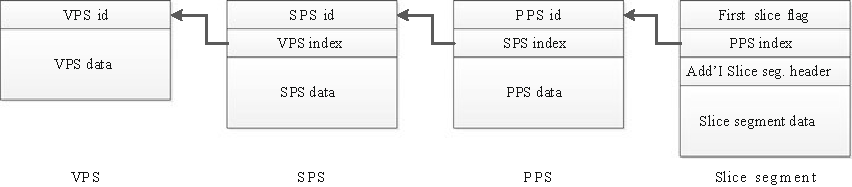
\includegraphics{NAL.pdf}
    \caption{H.265 网络适配层承载信息}
    \label{fig:NAL}
\end{figure}

为了保证硬件编码器的简洁,所实现的编码器仅输出视频编码层码流,将 NAL 单元的处理工作交给外部 CPU 进行处理,目前暂未实现。因此上位机接收到的码流无法直接进行解码,故解码模块有另一辅助程序参与,即 NAL 码流生成、提取模块。对相同配置参数软编码出的码流进行分析,提取出其中 NAL 码流将其拼接在 FPGA 输出码流的相应位置,得到的拼接文件即可在上位机正常解码,如 \ref{fig:FPGADemoBlock} 上位机解码部分所示。

\section{FPGA 原型验证结果}
% 照片
FPGA 原型验证平台在 XCZU15EG-2FFVB1156I 上映射占用的资源如表 \ref{tab:FPGAResource} 所示。
\begin{table}[hbt]
    \centering
    \caption{编码器 FPGA 映射资源使用情况}
    \label{tab:FPGAResource}
    \begin{tabular}{@{}lll@{}}
        \toprule
        资源   & 数量   & 使用率  \\ \midrule
        LUT    & 250660 & 73.45\% \\
        FF     & 9200   & 1.35\%  \\
        BRAMs  & 99     & 13.27\% \\
        DSP    & 463    & 13.11\% \\
        LUTRAM & 11680  & 3.42\%  \\ \bottomrule
    \end{tabular}
\end{table}

FPGA 原型验证平台实物如图 \ref{fig:FPGAphoto} 所示,图中包含摄像机、FPGA 开发板和主机显示器,其中摄像头与 FPGA 开发板上的 USB2UART 均通过 USB2.0 连接到显示器所对应的主机上。显示器中显示实时编、解码后的摄像头采集画面。
\begin{figure}[hbt]
    \centering
    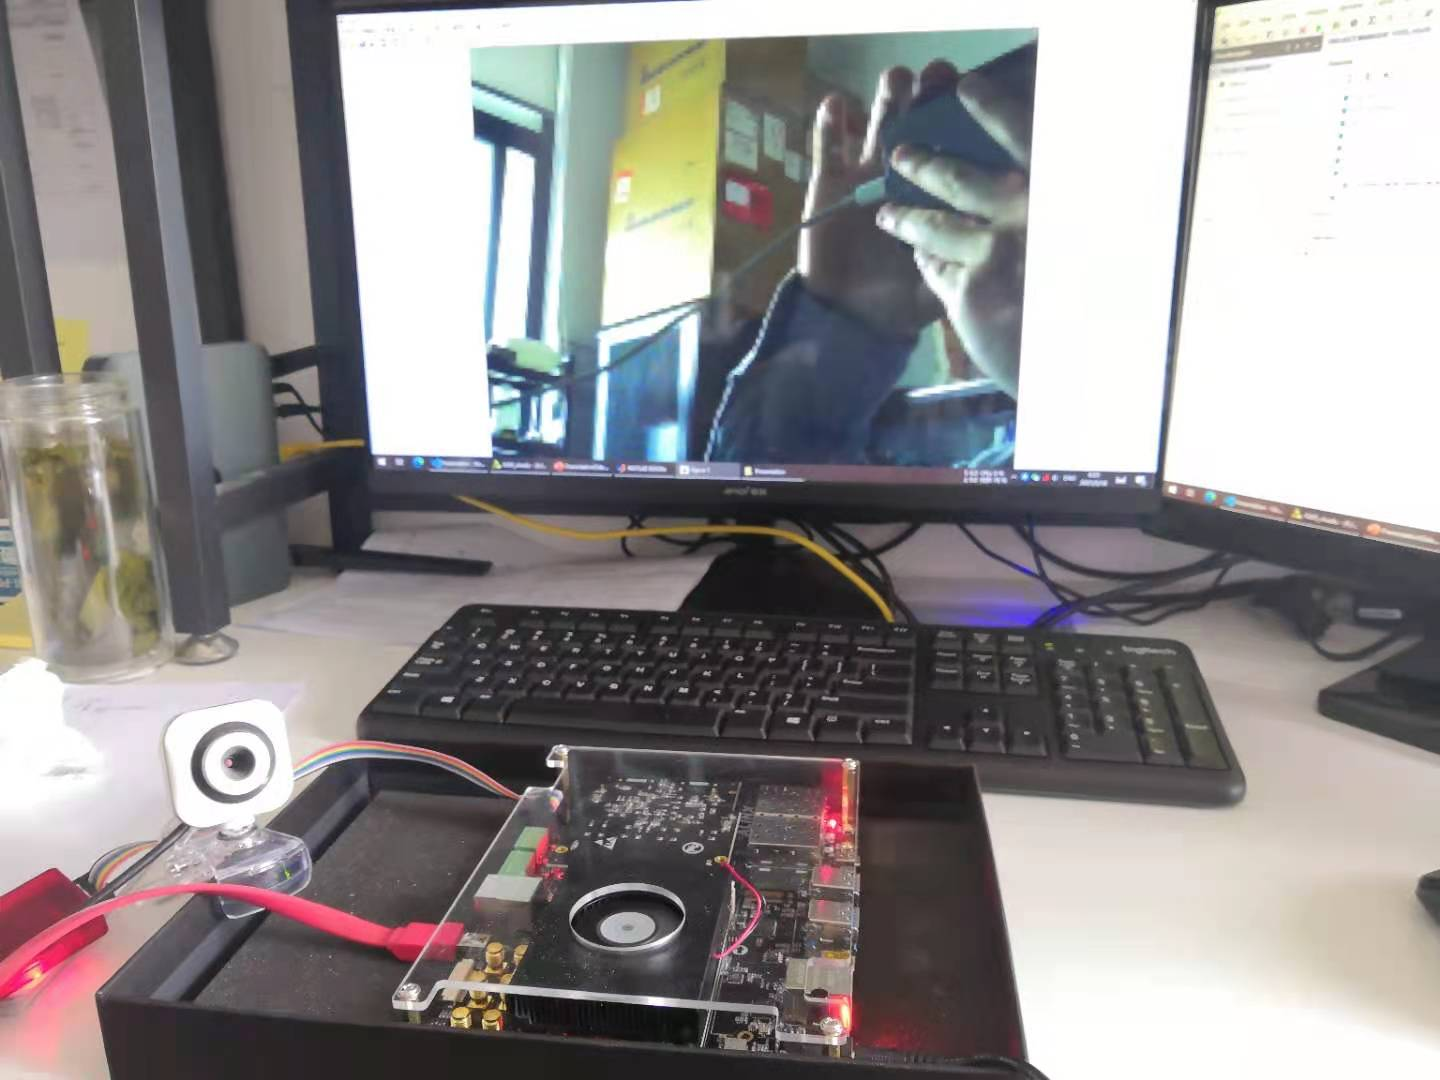
\includegraphics[scale=0.25]{FPGAphoto.jpg}
    \caption{FPGA 原型验证平台实物}
    \label{fig:FPGAphoto}
\end{figure}

% 说明摄影环境
与算法软件验证、行为级仿真验证不同,FPGA 原型验证采用编码实时摄像机获取的图像的方式,通过对比硬件编码输出码流的字节数进行验证。验证中选取了室内、建筑物内走廊、空旷室外和人像 4 个典型场景,验证结果如表 \ref{tab:FPGADemoTestTab} 所示。
\begin{table}[hbt]
    \centering
    \caption{FPGA 原型验证平台实际环境测试结果}
    \label{tab:FPGADemoTestTab}
    \begin{tabular}{@{}lcc@{}}
        \toprule
        \multicolumn{1}{c}{场景} & 码率     & 编码时间 \\ \midrule
        室内                     & -12.80\% & 118\%    \\
        建筑物内走廊             & -9.11\%  & 122\%    \\
        空旷室外                 & -12.91\% & 117\%    \\
        人像                     & -11.02\% & 118\%    \\ \midrule
        平均值                   & -11.46\% & 119\%    \\ \bottomrule
    \end{tabular}
\end{table}

验证结果普遍比测试序列优化程度更高,是因为测试序列大多属于较难编码的界面,编码块划分中很少出现大尺寸单元,不利于 L-BPIP 算法的发挥。

\section{本章小结}
本章介绍了课题研究过程中搭建的 FPGA 原型验证平台。使用 FPGA 进行原型验证灵活度高,验证结果可靠,且有利于软硬件协同设计、加快项目开发进度。
该验证平台由视频源、预处理模块、通信模块、硬件编码器和上位机解码模块组成。利用该平台可实时编码由视频源提供的图像信息,经映射入 FPGA 的硬件编码器编码后将码流传回上位机软解码,实时查看软解码结果正确与否即可对硬件编码器进行验证。